\documentclass{standalone}

\usepackage{tikz}
\usepackage{pgf}
\usetikzlibrary{positioning, chains, shapes.geometric, fit, shapes, arrows.meta, calc, backgrounds}

\begin{document}

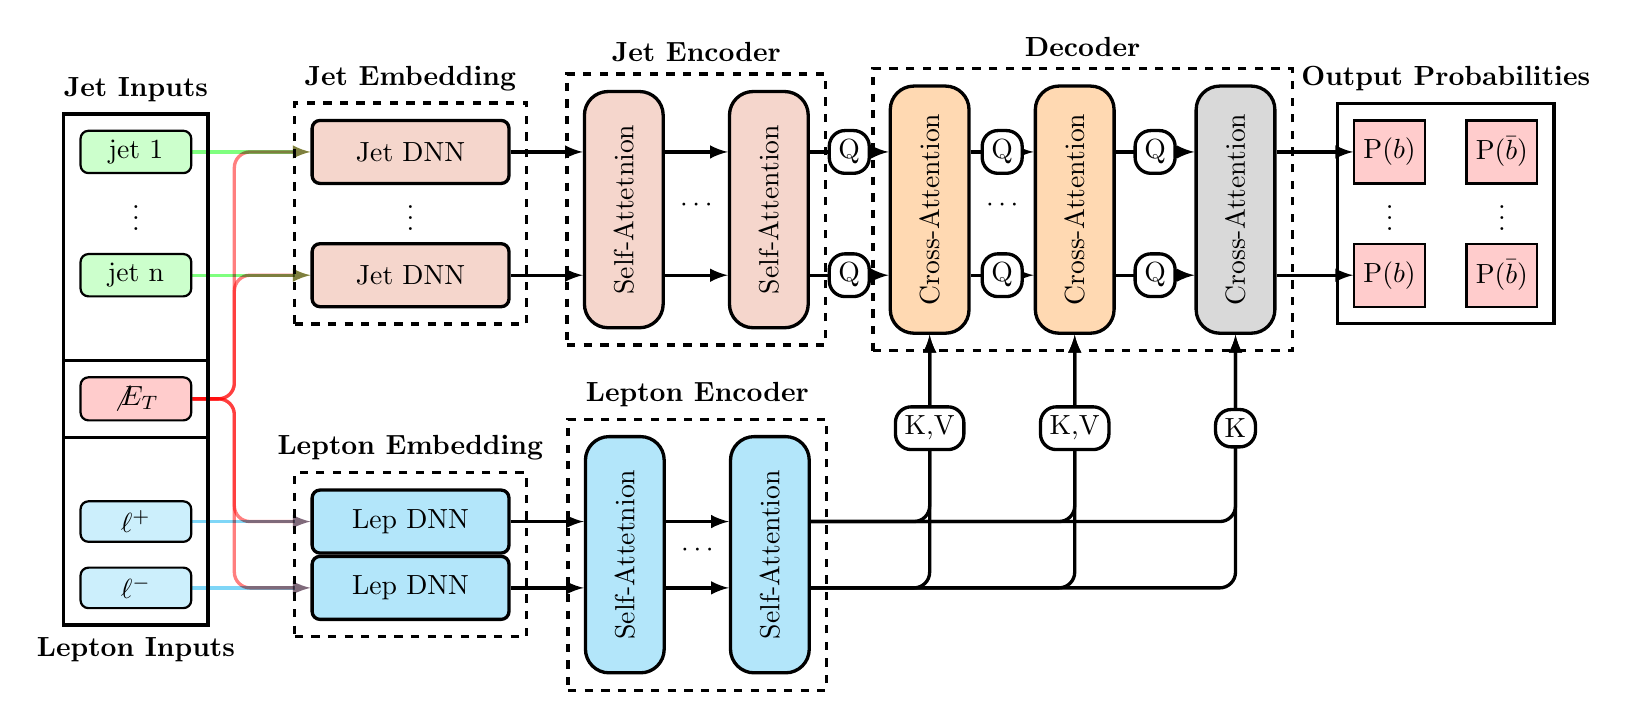
\begin{tikzpicture}[
      >=LaTeX,
      very thick,
      arrow/.style={
            -latex,
            very thick,
            rounded corners=0.2cm
      },
      block/.style={
            rectangle,
            fill=gray!10,
            rounded corners=3mm,
            draw,
            very thick
      },
      dnn_block/.style={
            rectangle,
            fill=blue!20,
            rounded corners=1mm,
            inner xsep=0em,
            inner ysep=0.25em,
            minimum height=1.4em,
            align=center,
            text width=2.5cm,
            draw,
            very thick
      },
      self_attention/.style={
            rectangle,
            fill=teal!20,
            rounded corners=3mm,
            inner xsep=1em,
            inner ysep=1em,
            align=center,
            draw,
            very thick
      },
      cross_attention/.style={
            rectangle,
            fill=orange!30,
            rounded corners=3mm,
            inner xsep=1em,
            inner ysep=1em,
            align=center,
            draw,
            very thick
      },
      input/.style={
            rectangle,
            minimum width=4em,
            rounded corners=1mm,
            draw,
            fill=green!20,
            thick
      },
      output/.style={
            rectangle,
            minimum height=0.8cm,
            draw,
            fill=red!20,
            thick
      },
      annotation/.style={
            font=\small\itshape,
            text=blue!70!black
      }
]

% Input nodes - Jets
\node[input,fill=green!20] (jet_1) {jet 1};
\node[input,fill=green!20, below=1cm of jet_1] (jet_n) {jet n};
\node[yshift=0.05cm] at ($(jet_1)!0.5!(jet_n)$) (jet_dots1) {$\vdots$};

% Input nodes - MET
\node[input,fill=red!20, below=1cm of jet_n] (met) {$\not{E}_T$};


% Input nodes - Leptons
\node[input,fill=cyan!20, below=1cm of met] (lepton_1) {$\ell^+$};
\node[input,fill=cyan!20, below=0.3cm of lepton_1] (lepton_2) {$\ell^-$};


% Jet Embeddings
\node[dnn_block, fill=green!20!red!20, right=1.5cm of jet_1, minimum height = 0.8cm] (jet_dnn_1) {Jet DNN};
\node[dnn_block, fill=green!20!red!20, right=1.5cm of jet_n, minimum height = 0.8cm] (jet_dnn_n) {Jet DNN};
\node[yshift=0.05cm] at ($(jet_dnn_1)!0.5!(jet_dnn_n)$) (jet_dnn_dots) {$\vdots$};

% Lepton Embeddings
\node[dnn_block, fill=cyan!30, right=1.5cm of lepton_1, minimum height = 0.8cm] (lep_dnn_1) {Lep DNN};
\node[dnn_block, fill=cyan!30, right=1.5cm of lepton_2, minimum height = 0.8cm] (lep_dnn_2) {Lep DNN};


% Jet Encoder
\node[self_attention, fill=green!20!red!20, 
      right=2cm of jet_dnn_dots, 
      minimum height=3cm, 
      minimum width=1cm] 
      (transformer_1) {\rotatebox{90}{Self-Attetnion}};

\node[self_attention, fill=green!20!red!20, 
      right=0.8cm of transformer_1, 
      minimum height=3cm, 
      minimum width=1cm] 
      (transformer_n) {\rotatebox{90}{Self-Attention}};
\node[yshift=0.05cm] at ($(transformer_1)!0.5!(transformer_n)$) (transformer_dots) {$\cdots$};

% Lepton Encoder
\coordinate (lepton_midpoint) at ($(lep_dnn_1)!0.5!(lep_dnn_2)+(0.2,0)$);

\node[self_attention, fill=cyan!30, 
      right=2cm of lepton_midpoint, 
      minimum height=3cm, 
      minimum width=1cm] 
      (lep_transformer_1) {\rotatebox{90}{Self-Attetnion}};

\node[self_attention, fill=cyan!30, 
      right=0.8cm of lep_transformer_1, 
      minimum height=3cm, 
      minimum width=1cm] 
      (lep_transformer_n) {\rotatebox{90}{Self-Attention}};
\node[yshift=0.05cm] at ($(lep_transformer_1)!0.5!(lep_transformer_n)$) (transformer_dots) {$\cdots$};


% Cross-Attention Layer
\node[cross_attention, fill=orange!30, 
      right=1cm of transformer_n, 
      minimum height=3cm, 
      minimum width=1cm] 
      (cross_attention_1) {\rotatebox{90}{Cross-Attention}};

\node[cross_attention, fill=orange!30, 
      right=0.8cm of cross_attention_1, 
      minimum height=3cm, 
      minimum width=1cm] 
      (cross_attention_2) {\rotatebox{90}{Cross-Attention}};
\node[yshift=0.05cm] at ($(cross_attention_1)!0.5!(cross_attention_2)$) (cross_attention_dots) {$\cdots$};

% Cross Attention Probabilities

\node[cross_attention, fill=gray!30, 
      right=1cm of cross_attention_2, 
      minimum height=3cm, 
      minimum width=1cm] 
      (cross_attention_probs) {\rotatebox{90}{Cross-Attention}};

% Output Probabilities

\node[output, right=10.7cm of jet_dnn_1] (output_b_1) {P($b$)};
\node[output, right=10.7cm of jet_dnn_n] (output_b_n) {P($b$)};
\node[yshift=0.05cm] at ($(output_b_1)!0.5!(output_b_n)$) (output_b_dots) {$\vdots$};

\node[output, right=0.5cm of output_b_1] (output_bbar_1) {P($\bar{b}$)};
\node[output, right=0.5cm  of output_b_n] (output_bbar_n) {P($\bar{b}$)};
\node[yshift=0.05cm] at ($(output_bbar_1)!0.5!(output_bbar_n)$) (output_bbar_dots) {$\vdots$};


% Arrows
\draw[arrow, color=green, opacity=0.5, blend mode=multiply] (jet_1) -- (jet_dnn_1);
\draw[arrow, color=green, opacity=0.5, blend mode=multiply] (jet_n) -- (jet_dnn_n);
\draw[arrow, color=red, opacity=0.5, blend mode=multiply] (met) -- ++(1.25,0) |- (jet_dnn_1);
\draw[arrow, color=red, opacity=0.5, blend mode=multiply] (met) -- ++(1.25,0) |- (jet_dnn_n);
\draw[arrow, color=red, opacity=0.5, blend mode=multiply] (met) -- ++(1.25,0) |- (lep_dnn_1);
\draw[arrow, color=red, opacity=0.5, blend mode=multiply] (met) -- ++(1.25,0) |- (lep_dnn_2);

\draw[arrow, color=cyan, opacity=0.5, blend mode=multiply] (lepton_1) -- (lep_dnn_1);
\draw[arrow, color=cyan, opacity=0.5, blend mode=multiply] (lepton_2) -- (lep_dnn_2);





% From Jet DNNs to Transformer
\draw[arrow] (jet_dnn_1.east) -- (jet_dnn_1.east -| transformer_1.west);
\draw[arrow] (jet_dnn_n.east) -- (jet_dnn_n.east -| transformer_1.west);



% Inside Transformer
\draw[arrow] (jet_dnn_1.east -| transformer_1.east) -- (jet_dnn_1.east -| transformer_n.west);
\draw[arrow] (jet_dnn_n.east -| transformer_1.east) -- (jet_dnn_n.east -| transformer_n.west);


% From Transformer to Cross-Attention
\draw[arrow](jet_dnn_1.east -| transformer_n.east) -- (jet_dnn_1.east -| cross_attention_1.west) node[midway, fill=white, draw, rectangle] {Q};
\draw[arrow] (jet_dnn_n.east -| transformer_n.east) -- (jet_dnn_n.east -| cross_attention_1.west)  node[midway, fill=white, draw, rectangle] {Q};

% Inside Cross-Attention
\draw[arrow] (jet_dnn_1.east -| cross_attention_1.east) -- (jet_dnn_1.east -| cross_attention_2.west) node[midway, fill=white, draw, rectangle] {Q};
\draw[arrow] (jet_dnn_n.east -| cross_attention_1.east) -- (jet_dnn_n.east -| cross_attention_2.west) node[midway, fill=white, draw, rectangle] {Q};

% From Leptons to Self-Attention
\draw[arrow] (lep_dnn_1.east) -- (lep_dnn_1.east -| lep_transformer_1.west);
\draw[arrow] (lep_dnn_2.east) -- (lep_dnn_2.east -| lep_transformer_1.west);

% Inside Lepton Transformer
\draw[arrow] (lep_dnn_1.east -| lep_transformer_1.east) -- (lep_dnn_1.east -| lep_transformer_n.west);
\draw[arrow] (lep_dnn_2.east -| lep_transformer_1.east) -- (lep_dnn_2.east -| lep_transformer_n.west);

% From Lepton Transformer to Cross-Attention
\draw[arrow] (lep_dnn_2.east -| lep_transformer_n.east) -|  ( cross_attention_1.south);
\draw[arrow] (lep_dnn_1.east -| lep_transformer_n.east) -|  ( cross_attention_1.south) node[near end, fill=white, draw, rectangle] {K,V};

\draw[arrow] (lep_dnn_2.east -| lep_transformer_n.east) -|  ( cross_attention_2.south);
\draw[arrow] (lep_dnn_1.east -| lep_transformer_n.east) -|  ( cross_attention_2.south) node[near end, fill=white, draw, rectangle] {K,V};

% From Cross-Attention to Cross-Attention Probs
\draw[arrow] (jet_dnn_1.east -| cross_attention_2.east) -- (jet_dnn_1.east -| cross_attention_probs.west) node[midway, fill=white, draw, rectangle] {Q};
\draw[arrow] (jet_dnn_n.east -| cross_attention_2.east) -- (jet_dnn_n.east -| cross_attention_probs.west) node[midway, fill=white, draw, rectangle] {Q};

% From Leptons to Cross-Attention Probs
\draw[arrow] (lep_dnn_2.east -| lep_transformer_n.east) -|  ( cross_attention_probs.south);
\draw[arrow] (lep_dnn_1.east -| lep_transformer_n.east) -|  ( cross_attention_probs.south) node[near end, fill=white, draw, rectangle] {K};

% From Cross-Attention Probs to Outputs
\draw[arrow] (jet_dnn_1.east -| cross_attention_probs.east) -- (output_b_1.west);
\draw[arrow] (jet_dnn_n.east -| cross_attention_probs.east) -- (output_b_n.west);




% Annotations for Cross-Attention
\node[fit=(jet_1)(jet_n)(met), 
      draw, 
      inner sep=0.2cm, 
      label=above:{\textbf{Jet Inputs}}] 
      (input_box) {};

\node[fit=(lepton_1)(lepton_2)(met), 
      draw, 
      inner sep=0.2cm, 
      label=below:{\textbf{Lepton Inputs}}] 
      (input_box) {};


\node[fit=(jet_dnn_1)(jet_dnn_n),
      draw, 
      dashed, 
      inner sep=0.2cm, 
      label=above:{\textbf{Jet Embedding}}] 
      (embedding_box) {};

\node[fit=(transformer_1)(transformer_n), 
      draw, 
      dashed, 
      inner sep=0.2cm, 
      label=above:{\textbf{Jet Encoder}}] 
      (transformer_box) {};

\node[fit=(lep_transformer_1)(lep_transformer_n), 
      draw, 
      dashed, 
      inner sep=0.2cm, 
      label=above:{\textbf{Lepton Encoder}}] 
      (lep_transformer_box) {};

\node[fit=(cross_attention_1)(cross_attention_2)(cross_attention_probs), 
      draw, 
      dashed, 
      inner sep=0.2cm, 
      label=above:{\textbf{Decoder}}] 
      (cross_attention_box) {};



\node[fit=(output_b_1)(output_b_n)(output_bbar_1)(output_bbar_n), 
      draw, 
      inner sep=0.2cm, 
      label=above:{\textbf{Output Probabilities}}] 
      (logit_box) {};

\node[fit=(lep_dnn_1)(lep_dnn_2), 
      draw, 
      dashed, 
      inner sep=0.2cm, 
      label=above:{\textbf{Lepton Embedding}}] 
      (lep_embedding_box) {};


\end{tikzpicture}
\end{document}
